\documentclass[12pt, english, a4paper]{extarticle}
\usepackage{cmap}
\usepackage[T2A]{fontenc}
\usepackage[utf8x]{inputenc}
\usepackage[vcentering,dvips]{geometry}
\usepackage[pdftex]{graphicx}
\usepackage{amssymb,amsfonts,amsmath,amsthm}
\usepackage{subfig}
\usepackage{hyperref}
\usepackage{float}
\usepackage{lscape}
\usepackage{array}
\usepackage{enumerate}
\usepackage{mdwlist}
\usepackage{textgreek}
\usepackage{fixltx2e}
\usepackage{longtable}
\usepackage{tabu}

\linespread{1.3}
\setlength{\parindent}{1cm}

\newcommand{\sub}[0]{\textsubscript}

\author{ Yaroslav Nechaev }
\title{ Feature Selection tool }

\begin{document}

\maketitle

\section{ Introduction }

Feature selection has become very important step in Natural Language Processing due to large amount of features that usually can be found in the datasets of the NLP-related problems. This is happening because it's typical to represent a piece of text as a feature vector, where each feature measures the "importance" of the corresponding term in the text (using various term frequency metrics). With a large amount of features we want to reduce their quantity by discarding irrelevant or redundant features. By selecting only relevant features we provide three main benefits for future analysis: improved model interpretability, shorter training times and reduced overfitting \cite{1}.

In this essay I will briefly review some of the related work on Feature Selection and describe main features of my tool.

\section{ Related Work }

One of the landmark systems in machine learning and data mining is The Waikato Environment for Knowledge Analysis (WEKA) \cite{2}. The WEKA provide a comprehensive collection of machine learning algorithms and related tools including various feature selection techniques. The library is open sourced and is available under the CC BY-SA 2.5 license.

Another major one is the Feature Selection Toolbox 3 \cite{3} by UTIA which is a standalone C++ library for feature selection. It contains wrappers, filters, hybrid methods, specialized methods for very high dimensional problems. Library is free for non-commercial use.

There is also a number of smaller tools can be found. One of them is Y.-W. Chen's et al. \cite{4} tool implementing a simple feature selection technique F-score. Zheng Zhao et al. \cite{5} maintain the repository containing 13 different algorithms and sample datasets for feature selection. Each algorithm is rated and performance report is available. Hanchuan Peng et al. \cite{6} researched applications of mRMR method related to gene selection.

\section{ Technical Description }

Feature selection algorithms generally fall into one of three categories: wrappers, filters and embedded methods \cite{1}. My tool implements two common filter algorithms: pointwise mutual information (PMI) and Pearson's chi-squared test (χ2). The application takes a LIBSVM file as an input, then ranks features based on their score and outputs the desired amount of the top scored features. 
Note that the tool assumes that features are binary: it assigns 1 if feature is present in the sample and 0 if it's not.

The application is written in Objective-C 2.0 with Automatic Reference Counting (ARC). Grand Central Dispatch is used for multi-threading. It will automatically select the best number of processes to handle the task.

\subsection{ PMI }

Pointwise mutual information \cite{7} is widely used to determine association between two discrete random variables. It is defined like this:

\begin{equation}
    PMI(x, y) = \log {\frac { p(x,y) }{ p(x)p(y) }}
\end{equation}

PMI is ranged as follows:
\begin{equation}
    -\infty \leq PMI(x, y) \leq min \left[ - \log { p(x) } , \log { p(y) }  \right]
\end{equation}

where PMI equals to zero if variables are independent, lower bound for never occuring together and upper bound for complete co-occurence. For our feature selection task, when we select only the most relevant features, we want this metric to be as far as possible from zero, meaning that the feature and the class are associated in some way.

The tool use this metric to score features against every class $c$, normalizes the result so it would be in $\left[-1,1\right]$, then summarize the score:

\begin{equation}
    s_i = \sum_{ c \in C } \left| \frac { PMI(f_i,c) }{ \log{p(f_i,c)} }  \right|
\end{equation}

where $s_i$ is the score for feature $f_i$.

\subsection{ $\chi^2$ test }

Pearson's chi-squared test \cite{8} is a statistical test to evaluate whether paired observations on two variables are independent of each other. For example, we could test if some words appears in texts on certain topic more likely than on the other topics, or we could check if the certain diet increases the likelihood of the certain illness.
The value of the test statistic is:

\begin{equation}
    X^2 = \sum_{i,j} \frac { \left( O_{ij} - E_{ij} \right)^2 } { E_{ij} }
\end{equation}

Where values $O_{ij}$ are observed values from the contingency table \cite{9}, $E_{ij}$ are expected values. For feature selection task we have two variables — particular feature with two outcomes (feature is in sample or it is not) and class. This way we have $2\times\left|C\right|$ contingency table (see Table 1). The tool constructs this table and calculates the metric.

\begin{table}[h]
  \centering
  \begin{tabular}{ | c | c | c | c | c | }
    \hline
    & $C_1$ & $C_2$ & $C_3$ & Total \\ \hline
    $f_i$ & 4 & 5 & 6 & 15 \\ \hline
    $\neg f_i$ & 7 & 8 & 9 & 24 \\ \hline
    Total & 11 & 13 & 15 & 39 \\
    \hline
  \end{tabular}
  \caption{Example of contingency table for 3 classes}
\end{table}

\subsection{ Code organization }

Code consists of main file ($main.m$) and four classes ($ChiSquaredEvaluator$, $Evaluator$, $PMIEvaluator$, $DatasetCollector$). Main file contains all IO logic and also parses input in LIBSVM format. 

$DatasetCollector$ is a helper class used for iterative assembling of the sample info into the NSDictionary. 

$Evaluator$ is an abstract class with the main metric calculation routines, including the multi-threading support. Other two classes ($*Evaluator$) extend $Evaluator$ class and implement particular method. This method takes a feature info with some general precomputed statistics about the original data as an input and outputs the score of the particular feature. 

\begin{figure}[h]
\centering
    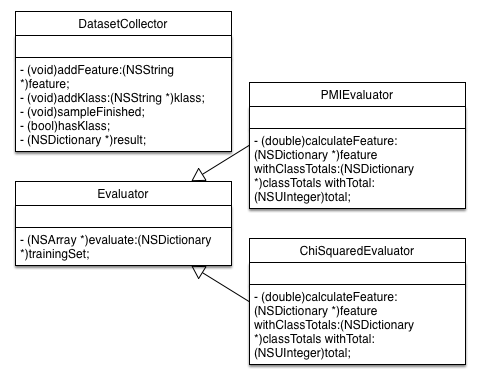
\includegraphics[scale=0.55]{code_diagram.png}
    \caption{Code diagram}
    \label{fig_schema}
\end{figure}

\renewcommand\refname{ }
\section{ References }
\nocite{*}
\bibliographystyle{unsrt}
\bibliography{ml}

\end{document}
